\documentclass[crop,tikz]{standalone}% 'crop' is the default for v1.0, before it was 'preview'
\usepackage{physics}
\usepackage{tikz}
%\usepackage[outline]{contour} % glow around text
\usetikzlibrary{arrows.meta} % for arrow size
\tikzset{>=latex}
\colorlet{mydarkblue}{blue!40!black}
\colorlet{myblue}{blue!70!black}
\colorlet{myred}{red!65!black}
\colorlet{myorange}{orange!85!black!90}
\colorlet{vcol}{green!45!black}
\colorlet{metalcol}{blue!25!black!20!white}
\tikzstyle{metal}=[draw=metalcol!30!black,rounded corners=0.1,top color=metalcol,bottom color=metalcol!80!black,shading angle=10]
\tikzstyle{vvec}=[->,very thick,vcol,line cap=round]
\tikzstyle{force}=[->,myred,very thick,line cap=round]
\tikzstyle{width}=[{Latex[length=3,width=2.5]}-{Latex[length=3,width=2.5]}]
\tikzstyle{myperp}=[x={(0.72cm,-0.08cm)},y={(0.40cm,0.30cm)},z={(0,1cm)}]
\def\tick#1#2{\draw[thick] (#1)++(#2:0.12) --++ (#2-180:0.24)}
%\usetikzlibrary{...}% tikz package already loaded by 'tikz' option
\begin{document}
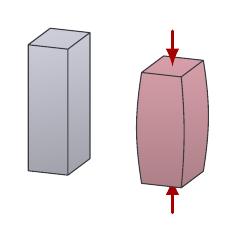
\begin{tikzpicture}[myperp]

\def\W{0.7}     % side width
\def\H{1.6}     % total height
\def\F{0.28*\H} % force magnitude
% \begin{tikzpicture}[myperp]
  \draw[metal]
    (0,0,0) --++ (\W,0,0) --++ (0,0,\H) --++ (-\W,0,0) -- cycle
    (\W,0,0) --++ (0,\W,0) --++ (0,0,\H) --++ (0,-\W,0) -- cycle
    (0,0,\H) --++ (\W,0,0) --++ (0,\W,0) --++ (-\W,0,0) -- cycle;

    \def\h{0.88*\H}
  \draw[force] (\W/2+2,\W/2,-\F) --++ (0,0,\F);
  \draw[metal,top color=metalcol!78!red,bottom color=metalcol!78!red!80!black]
    (2,0,0) --++ (\W,0,0) to[out=85,in=-85]++ (0,0,\h) --++ (-\W,0,0) to[out=-99,in=99] cycle
    (\W+2,0,0) --++ (0,\W,0) to[out=81,in=-81]++ (0,0,\h) --++ (0,-\W,0) to[out=-85,in=85] cycle
    (2,0,\h) --++ (\W,0,0) --++ (0,\W,0) --++ (-\W,0,0) -- cycle;
  \draw[force] (\W/2+2,\W/2,\h+\F) --++ (0,0,-\F);

\end{tikzpicture}
\end{document}